\section{Methodology}\label{sec:METHOD}
%% this part will hold all necessary data for our method reproduction
%% we explicitly explain what decision were made, what libraries and hardware were used

%% below you see some examples of how to embed images and tables



In \cite{AmbientApproxHyper} authors use B-splines to approximate a function on a hypersurface. They first extend a hypersurface with a neighbourhood, then use B-splines to approximate function in the neighbourhood and then restrict.
% пипец сложно и непонятно, но там есть ссылка на хорошую статью вроде бы:

TBD \cite{ScatteredDataInterpolation}



MNIST \cite{mnist}

100LEAVES \cite{100leaves}





%% how to embed image for 2 columns
% \begin{figure*}[ht]
% 	\normalsize
%     \centering
%     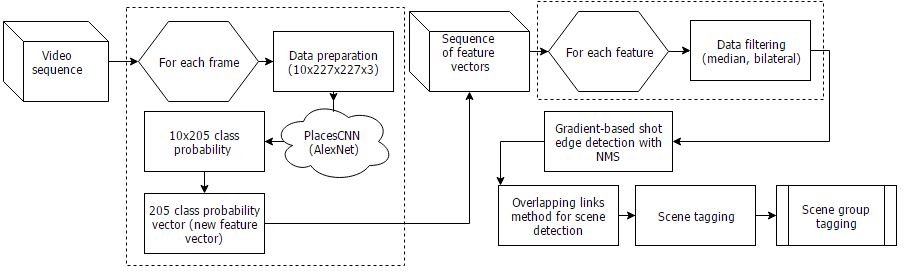
\includegraphics[width=6.3in]{images/Fig1.png}
%     \caption{The title}
%     \label{fig:workflow}
% \end{figure*}

% An overview of the proposed approach is shown in figure \ref{fig:workflow}.

% %% how to embed 1-column image
% \begin{figure}
%     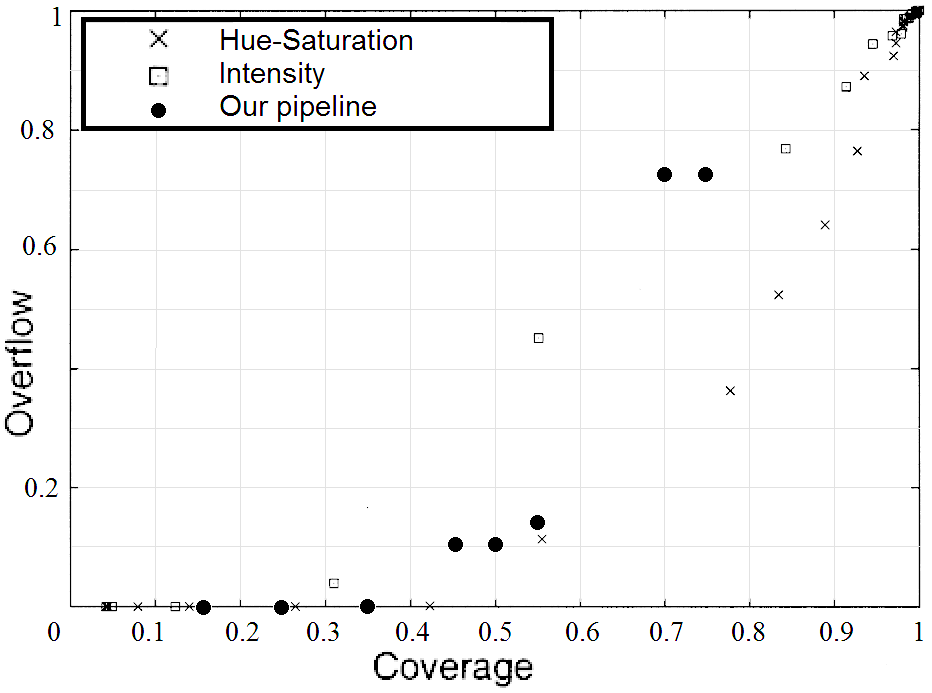
\includegraphics[width=3.3in]{images/Fig2.png}
%     \caption{Comparison of coverage and overflow metrics values for our pipeline with original paper}
%     \label{fig:cov-over}
% \end{figure}

% This is how we refer this image \ref{fig:cov-over}.


%% how to embed table
% \begin{table}
% \caption{Oversegmentation with different filters for top achieved accuracies for 30fps dataset}
% \label{tb:oversegment}
% \centering
% \begin{tabular}{ | c | p{16mm} | p{16mm} | c | }
% \hline
% \textbf{Filter} & \textbf{Param.} & \textbf{Edge det. \newline accuracy} & \textbf{Oversegm.} \\
% \hline
% No filter & -- & 0.929 & 10.571 \\
% \hline
% Median & $W=3$ & \textbf{0.982} & 13.5 \\
% \hline
% Median & $W=5$ & 0.964 & \textbf{8.75} \\
% \hline
% Bilateral & ${\sigma}_{g}=1,\newline {\sigma}_{f}=0.1$ & 0.964 & 12.5 \\
% \hline
% Bilateral & ${\sigma}_{g}=1,\newline {\sigma}_{f}=0.3$ & 0.964 & 13.732 \\
% \hline
% \end{tabular}
% \end{table}

This is how we refer tables: ~\ref{tb:oversegment}.